\documentclass[a4paper,onecolumn,superscriptaddress,10pt]{compositionalityarticle}
\pdfoutput=1
\usepackage{silence}
\WarningFilter{caption}{Unknown document class (or package)}
\usepackage[font=small,skip=5pt,style=base]{caption}
\usepackage[utf8]{inputenc}
\usepackage[english]{babel}
\usepackage[T1]{fontenc}
\usepackage{amsmath}
\usepackage{hyperref}
\usepackage{pgf-pie}
\usepackage{tikz}
\usepackage{pgfplots}
\usepackage{bookmark}
\pgfplotsset{compat=1.18}
\usepackage{lipsum}
\usepackage{booktabs}
\usepackage{siunitx}

\newtheorem{theorem}{Theorem}
\usetikzlibrary{positioning}
\makeatletter
\providecommand{\@shorttitle}{Vecno}
\makeatother

\begin{document}

\title{Vecno Blockchain Whitepaper}
\date{25/12/2025}
\author{
    {\small Whitepaper v.0.0.1 --- Written By \small \href{https://github.com/Yooshikii}{Yoshiki}}
}
\email{support@vecnofoundation.org}
\homepage{https://vecnofoundation.org}
\maketitle

\begin{abstract}
    Vecno is a blockchain platform designed to overcome the limitations of existing consensus mechanisms by using Proof of History (PoH), blockDAGs, and an optimized consensus structure. In certain cases, Vecno will also rely on Proof of Work (PoW) to validate transactions, ensuring maximum security and integrity. This unique combination introduces a high-performance, low-energy system that maintains decentralization while offering scalability, speed, and security. This innovative approach challenges the dominance of Proof of Work and Proof of Stake models by providing a more efficient alternative for real-time transaction validation.

    Vecno is not merely an incremental improvement on existing blockchain models; it re-envisions blockchain infrastructure to support a decentralized, fair, and scalable digital economy. At the heart of this mission is the Vecno Foundation, responsible for the operation and maintenance of the Vecno blockchain and its associated services. The Foundation also spearheads the development and implementation of new functions and continuous improvements, providing robust support for both users and developers.

    In addition to technical innovation, the Vecno Foundation leads marketing efforts to promote the platform and collaborates with other organizations and projects in the broader cryptocurrency and blockchain ecosystems. Proudly, Vecno is the first company in Norway to develop blockchain technology, marking a significant achievement in the nation's technological advancements.

\end{abstract}

\vspace{7cm}

\footnotesize{\textit{Vecno builds upon lessons learned from earlier blockchain innovations such as Bitcoin and Ethereum, while overcoming their limitations. By implementing PoH, BlockDAGs and occasionally PoW alongside practical use-cases, Vecno provides a strong foundation for decentralized applications, digital assets, and secure financial systems. This whitepaper outlines Vecno’s core philosophy, technical advancements, and future roadmap.}}

\newpage

\section{Native Asset}

The Vecno network operates with its native asset, symbol \texttt{VE}, which serves as the blockchain's gas for executing transactions, smart contracts, and securing the network. \texttt{VE} has 8 decimal places to support high-precision transfers and prevent rounding errors. The total supply of \texttt{VE} will be capped at 200 million, with the supply expected to reach its maximum within 50 years. This ensures controlled inflation that aligns with the growth of the platform, serving as a safeguard for the long-term stability of the currency. Block rewards follow a gradual reduction model, where the reward per block decreases over time according to the formula:

\[
\text{current block reward} = \text{Initial Block Reward} \times {\left( \frac{1}{2} \right)}^{\frac{\text{xMonth}}{24}}
\]
\vspace{0.3cm}

Initially, the block reward is set to 2 \texttt{VE} per block. Vecno uses a gradual reduction mechanism that ensures rewards decrease steadily while maintaining sufficient incentives for network participants. This formula reflects a reduction in block rewards by half every 24 months (or approximately two years), ensuring that validators are continuously incentivized while allowing for controlled and predictable emissions. To use this in an example we calculate the block reward after 120 months with an initial block reward of 2, we use the formula:
\vspace{0.4cm}

\[
2 \times {\left( \frac{1}{2} \right)}^{\frac{120}{24}}
\]

\vspace{0.3cm}
\[
{\left( \frac{1}{2} \right)}^{\frac{120}{24}} = 0.03125
\]

\vspace{0.3cm}

\[
\text{current block reward} \approx 2 \times 0.03125 \approx 0.0625
\]


\vspace{0.3cm}

After 10 years, the block reward will be reduced to \textbf{0.0625} \texttt{VE} per block. This gradual reduction ensures a predictable and fair distribution of rewards over time, while also preserving the long-term stability of the network by preventing inflation from devaluing \texttt{VE}. 
\vspace{0.3cm}

\begin{figure}[h!]
    \centering
    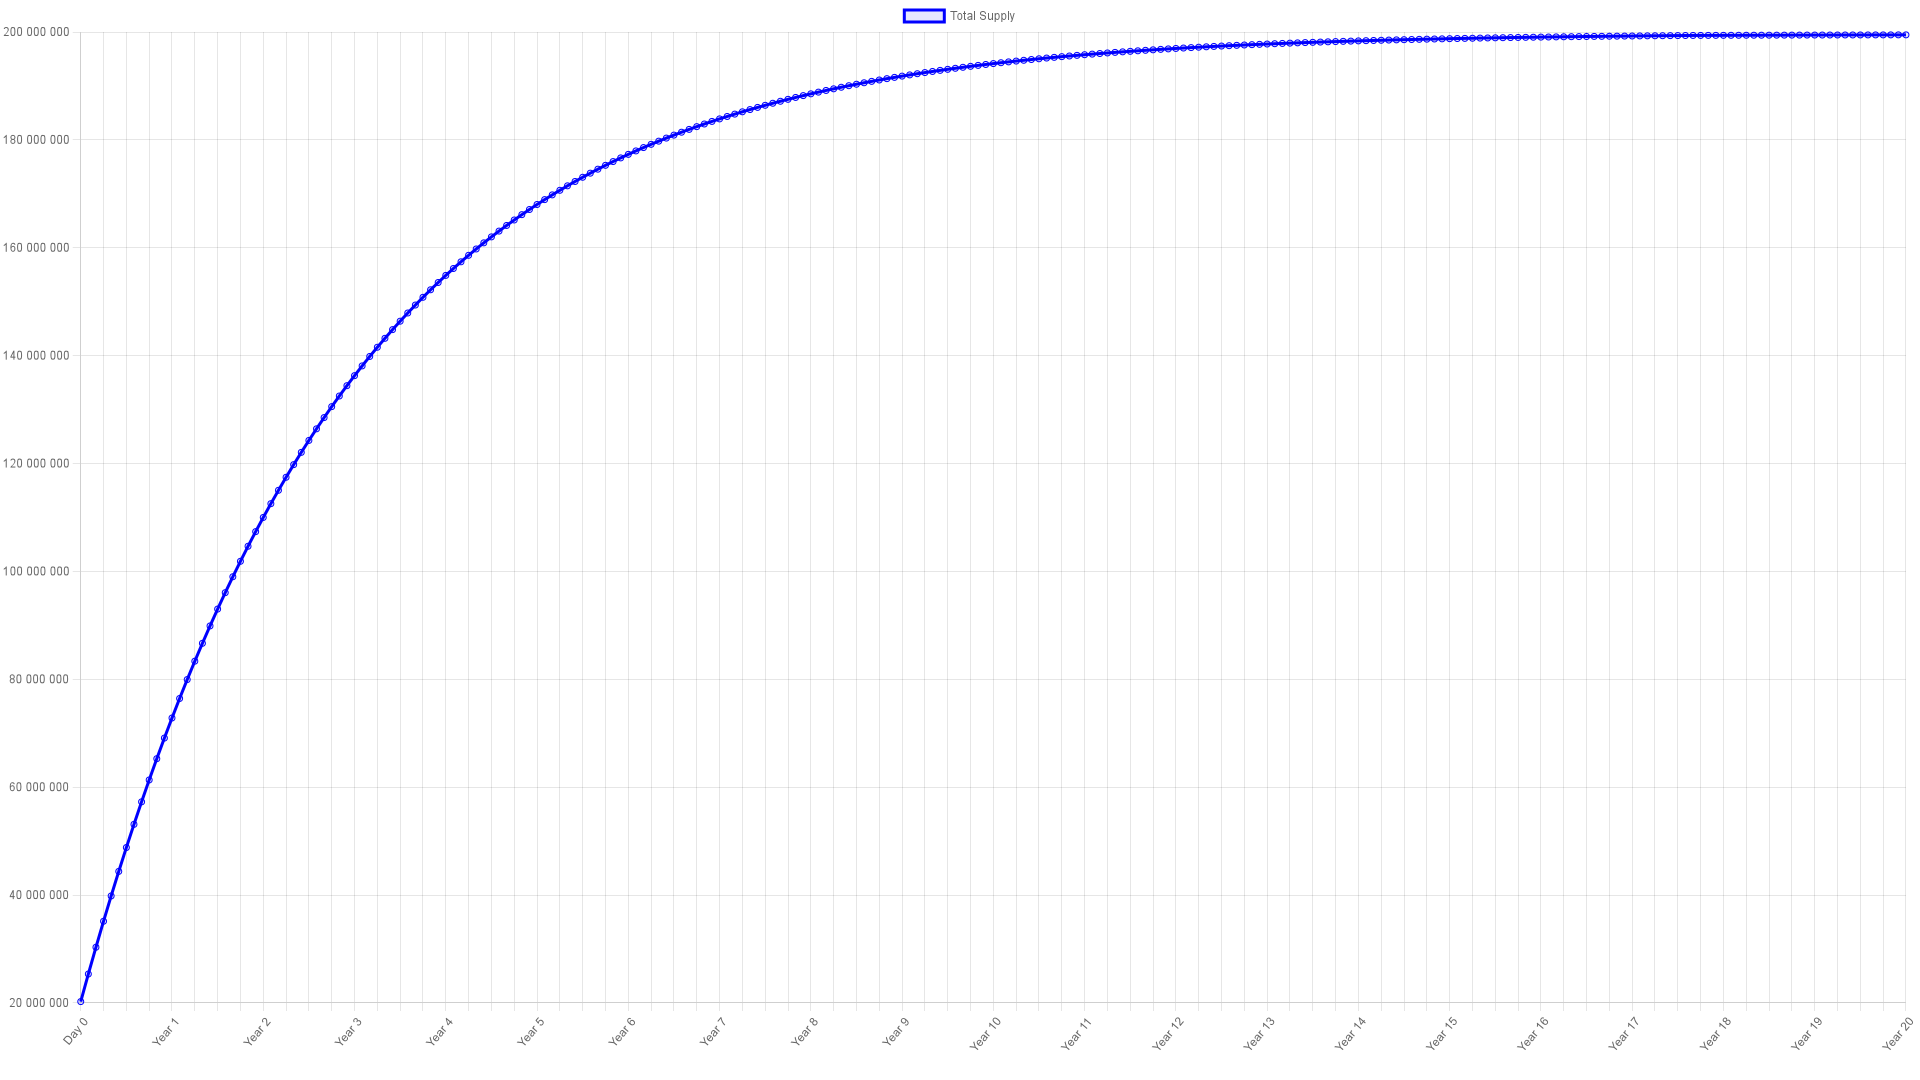
\includegraphics[width=\textwidth]{chart.png}
    \caption{Block Reward Emissions}\label{fig:chart}
\end{figure}

The block rewards will continue to decrease until they hit 0.001 \texttt{VE} per block, which will occur in around 22 years. By that time, 199.5 million \texttt{VE}, around 99 percent of the total supply will have been mined. Using the formula, the last 0.1 percentages will take another 30 years to be fully mined. This steady reduction ensures that inflation is kept in check, and long-term network sustainability is maintained. Once the total supply of 200 million \texttt{VE} has been reached, block rewards will stop entirely. At that point, validators will be compensated solely through transaction fees, ensuring continued security and network maintenance. This steady reduction ensures that inflation is kept in check, and long-term network sustainability is maintained. Transaction fees on the Vecno network are dynamically adjusted to maintain network efficiency and balance validator incentives. A fair and transparent fee structure ensures that both validators and users benefit from the network's operation. These measures allow Vecno to scale while aiming for equitable participation from its users.

\vspace{0.3cm}

\subsection{Commodity}\label{sec1.1}

The \texttt{VE} asset functions as more than just a utility for the Vecno network; it is regarded as a commodity due to its inherent value derived from its utility, scarcity, and decentralized nature. Similar to commodities like oil or precious metals, \texttt{VE} has real-world economic applications within the Vecno ecosystem and plays a critical role in the network's operations. It is the necessary `fuel' for executing smart contracts, processing transactions, and securing the network through validator participation.
However, it is important to note that \texttt{VE} is not considered an investment. Its primary function is to serve the operational needs of the network, facilitating transactions and providing utility within the Vecno ecosystem. \texttt{VE} holders engage with the network to secure the blockchain, and utilize its decentralized applications, rather than seeking speculative financial returns.

The supply of \texttt{VE}, capped at 200 million, ensures that as demand for its utility increases, its scarcity will drive value over time. This economic model, combined with the controlled release of new \texttt{VE} through diminishing block rewards, mirrors traditional commodities in that the supply is limited, and extraction becomes more difficult over time.
In addition, \texttt{VE}’s decentralized nature ensures that no central authority controls the currency. Its role in governing the network and compensating validators means that it serves as a tangible, tradeable asset with a clear value proposition in the broader cryptocurrency markets. This blend of functionality, scarcity, and economic relevance qualifies \texttt{VE} as a commodity, ensuring its place as a valuable and essential asset within both the Vecno network and the wider blockchain economy.

\subsection{MemHash Algorithm}\label{sec1.2}

The MemHash algorithm is a custom Proof-of-Work mechanism designed specifically for the Vecno blockchain. Its goal is to secure the network in a way that is fair, energy-efficient in context, and resistant to domination by specialized hardware (like ASICs). This promotes true decentralization by allowing anyone with a standard CPU or GPU to participate in mining effectively. 

MemHash is built on top of BLAKE3, one of the fastest and most secure cryptographic hash functions available today. BLAKE3 is much quicker than older functions like SHA-256 (used in Bitcoin) or Keccak (used in old Ethereum), while providing strong protection against attacks.
To make the algorithm memory-hard, MemHash adds layers that require accessing a moderate amount of memory in an unpredictable way. This slows down specialized hardware (which excels at pure computation) but doesn't heavily impact regular computers. The result is a balanced PoW that encourages broad participation.
MemHash takes three inputs to create a unique puzzle for miners: \\ (i) The previous block's hash (32 bytes, linking to the blockchain history). \\ (ii) A timestamp (to incorporate time). \\ (iii) A nonce (a number the miner tries different values for, to solve the puzzle).

The algorithm runs in several phases: \\ (i) Initialization (Setup Phase): A small substitution box (S-box, 64 bytes) is generated using BLAKE3 seeded from the input hash. This S-box acts like a random lookup table unique to each block. The number of rounds (between 16 and 23) is calculated dynamically using BLAKE3 on the input hash and timestamp. This adds variability so no two blocks have exactly the same difficulty structure. An initial 256-bit state (8 × 32-bit words) is derived directly from the input hash. \\ (ii) Pre-Mixing Phase (Intense Hashing Warm-Up): The initial state is repeatedly hashed with BLAKE3 (twice the number of rounds, split into two identical loops). After each BLAKE3 hash, simple bit manipulations are applied (XORing certain bytes together) to mix the data further. This phase thoroughly scrambles the state using fast hashing, creating a strong starting point.
\\ (iii) Main Mixing Phase (Memory-Hard Core): For each round (16–23 times): For each of the 8 state words: A BLAKE3 hash is computed using the current word, round number, and nonce. This creates data-dependent values. The result is XOR-mixed with the full current state. The state word is updated by XORing, then applying one of four operations (add, subtract, rotate, or XOR) chosen pseudo-randomly. Finally, the word's bytes are used as offsets to look up values in the unique S-box, replacing the word with the looked-up bytes interpreted as a new 32-bit value. These unpredictable S-box lookups make the process memory-hard: the algorithm must frequently access scattered memory locations, which is efficient on CPUs/GPUs but costly for ASICs. \\ (iv) Finalization: After all rounds, the state is converted back to bytes. One last bit manipulation is applied. A final BLAKE3 hash is computed on the result to produce the 256-bit output hash.

Miners repeatedly increment the nonce (and sometimes adjust the timestamp slightly) until the final hash meets the network's difficulty target (e.g., starts with enough zero bits). This trial-and-error process requires real computational work, securing the chain. By combining fast BLAKE3 iterations with data-dependent memory accesses and variable rounds, MemHash is tunable, secure, and ASIC-resistant while remaining simple to implement and verify.

\subsection{Comparison with Traditional Algorithms}
MemHash offers clear advantages over classic PoW algorithms like SHA-256 (Bitcoin) or Keccak (pre-PoS Ethereum):

\begin{itemize}
\item \textbf{Much Faster}: BLAKE3 can process data at speeds up to 10 GB/s per core—far exceeding SHA-256 (~0.5 GB/s) or Keccak (~0.3 GB/s). This enables quicker puzzle solving and validation.
\item \textbf{Memory-Hard Design}: Unlike pure computation-heavy algorithms, MemHash's S-box lookups deter ASIC dominance, keeping mining accessible to consumer hardware.
\item \textbf{Stronger Security}: BLAKE3 provides 256-bit security with a modern design resistant to known attacks, including better margins against future threats like quantum computing.
\item \textbf{Lower Risk of Bugs}: BLAKE3's simple, well-audited structure reduces implementation vulnerabilities.
\end{itemize}

When paired with Proof-of-History and BlockDAG, MemHash enables Vecno to deliver high security without the full energy cost of constant traditional PoW.

\newpage

\section{Vecno Foundation}

The Vecno Foundation is a registered company that manages the daily operations, development, and overall maintenance of the Vecno blockchain and its associated services. The Foundation plays a pivotal role in ensuring the blockchain's functionality, security, and scalability, while also driving user engagement and ecosystem growth.
\\Vecno Foundation is registered with the organisation number 933 980 073, for more information about the company visit the \href{https://virksomhet.brreg.no/en/oppslag/enheter/933980073}{Brønnøysund Register Centre}.

\vspace{0.3cm}

\subsection{Membership and Services}\label{sec2.1} 

Joining the Vecno Foundation as a member provides individuals or organizations with partial ownership and access to exclusive services tailored to enhance participation in the Vecno ecosystem. Membership requires an initial deposit equivalent to 1,000 USD in Vecno coins and an annual contribution of 100 USD in Vecno coins. Members gain the following benefits:\\ (i) Regular Progress Updates: Weekly reports providing detailed insights into the Vecno blockchain’s advancements and ongoing developments.\\ (ii) Comprehensive Educational Resources: Unlimited access to learning materials designed to expand understanding of Vecno and blockchain technology.\\ (iii) Continuous Technical Assistance: Round-the-clock support services to address any technical issues members may encounter.\\ (iv) Annual Profit Distribution: Eligibility to receive a portion of the Vecno Foundation’s yearly profits.\\ (v) Governance Participation: The right to vote on key decisions affecting Vecno’s operations, providing a decentralized governance model.

\vspace{0.3cm}

\subsection{Fees and Revenue}\label{sec2.2}

The Vecno Foundation manages the blockchain’s financial resources to ensure long-term sustainability and growth. Revenue is generated through various fees, partnership fees, membership fees, and profit-sharing. These funds are allocated to the following key areas:\\ (i) DApp Development Support: Comprehensive support is offered for developers building decentralized applications (DApps) on the Vecno network, from concept to deployment.\\ (ii) Management: A dedicated team handles day-to-day blockchain operations, ensuring smooth functionality and addressing any operational needs.\\ (iii) Community Onboarding: The Foundation offers training programs for new members, ensuring they can contribute to and benefit from the Vecno ecosystem.

\vspace{0.3cm}


\subsection{Treasury}\label{sec2.3}

The Vecno Foundation manages the blockchain's financial resources with a total premine of 15 million coins, representing 7.5 percent of the total supply. Here's how these funds are distributed:\\ (i) Community Donation Offering: 10 million coins are dedicated to the community, aiming to raise capital and increase community involvement in the project.\\ (ii) Vecno Foundation Development Fund: 3 million coins are set aside for the Vecno Foundation to cover future development costs, operational expenses, and other foundational activities.\\ (iii) Vecno Foundation Listing Fund: 1 million coins are set aside for the Vecno Foundation to cover listing costs, which will be paired with some of the capital raised from the community fund.\\ (iiii) Vecno Foundation Team Treasury: 1 million coins which is reserved for the Vecno Blockchain Development team and founders.

\vspace{0.3cm}

\begin{center}\label{fig:premine}
    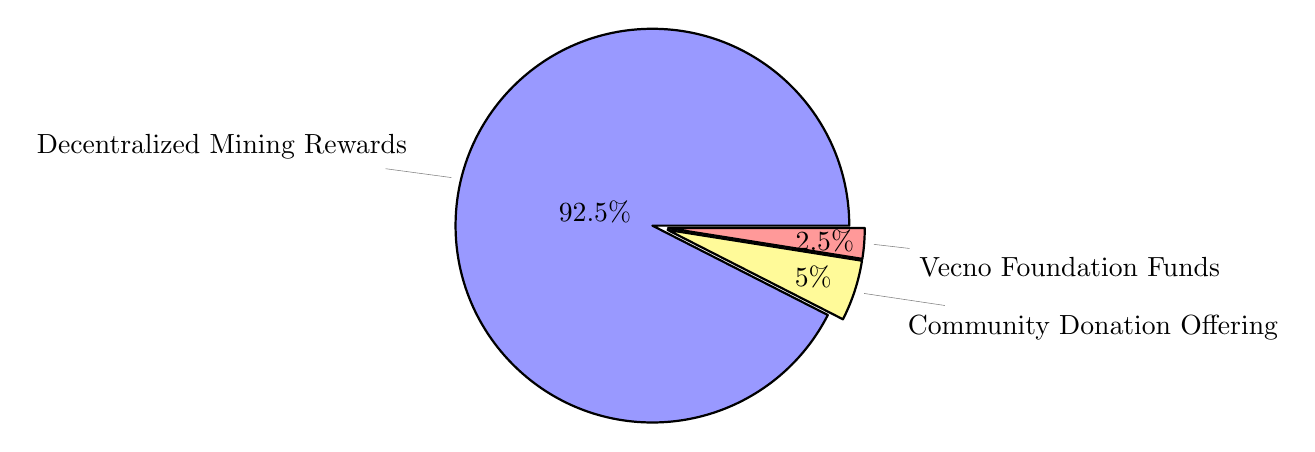
\begin{tikzpicture}
        \pie[
            text=pin,
            radius=2.5,
            color={blue!40, yellow!40, red!40},
            sum=100,
            explode=0.1
        ]{
            92.5/Decentralized Mining Rewards,
            5/Community Donation Offering,
            2.5/Vecno Foundation Funds
        }
    \end{tikzpicture}
\end{center}
\vspace{0.3cm}

The premine was mined in the wallet with the address:

\vspace{0.3cm}

\href{https://vecnoscan.org/addresses/vecno:qp8dhhdyltaxwhu7c24gyvzs7jg34fwggvqp62zsgfvnfkqq3xdukynlm9uw5}{vecno:qp8dhhdyltaxwhu7c24gyvzs7jg34fwggvqp62zsgfvnfkqq3xdukynlm9uw5}


\vspace{0.3cm}

This allocation of the premine helps with growth, sustainability, and efficiency of the Vecno blockchain ecosystem. The following table outlines the structure of the Community Donation Offering, which operates on a \textbf{first-come, first-served} basis. Participants donate USDT (Tether) to receive airdropped coins at the specified price tiers. The price per coin increases as each tier is filled, starting at \$0.020 for the first 1,000,000 coins and rising incrementally to \$0.200 for the final 1,000,000 coins.

\begin{table}[h]
\centering
\caption{Donation Tiers}
\begin{tabular}{S[table-format=7.0] S[table-format=1.3] S[table-format=6.2]}
\toprule
{Number of Coins} & {Price per Coin (USD)} & {Total Raised (USD)} \\
\midrule
1000000 & 0.020 & 20000.00 \\
500000  & 0.030 & 15000.00 \\
500000  & 0.040 & 20000.00 \\
500000  & 0.050 & 25000.00 \\
500000  & 0.060 & 30000.00 \\
500000  & 0.070 & 35000.00 \\
500000  & 0.080 & 40000.00 \\
500000  & 0.090 & 45000.00 \\
500000  & 0.100 & 50000.00 \\
500000  & 0.110 & 55000.00 \\
500000  & 0.120 & 60000.00 \\
500000  & 0.130 & 65000.00 \\
500000  & 0.140 & 70000.00 \\
500000  & 0.150 & 75000.00 \\
500000  & 0.160 & 80000.00 \\
500000  & 0.170 & 85000.00 \\
500000  & 0.180 & 90000.00 \\
500000  & 0.190 & 95000.00 \\
1000000 & 0.200 & 200000.00 \\
\midrule
\textbf{10000000} & & \textbf{\$1010000.00} \\
\bottomrule
\end{tabular}
\end{table}

\vspace{1cm}

\begin{itemize}
    \item Total coins airdropped: 10,000,000
    \item Total funds raised: \$1,010,000.00 (in USDT)
\end{itemize}

\vspace{0.5cm}

The majority of the funds raised through donations, totaling \$1,010,000.00 in USDT, is allocated to \textbf{listings and marketing}. \$60,000.00 will be dedicated to \textbf{operational costs} to support the project's ongoing activities and infrastructure.

\subsection{Development Goals}\label{sec2.4}

The Vecno Foundation is focused on pioneering a blockchain that sets new benchmarks for performance, accessibility, and innovation. The development goals prioritize creating a versatile platform that supports diverse use cases while advancing Norway’s role in blockchain technology. These objectives drive the Foundation’s roadmap to enhance the Vecno ecosystem through cutting-edge technical advancements and user-focused solutions.

Vecno’s codebase originates from Kaspa, a high-performance blockchain built in Rust, leveraging its BlockDAG structure and GHOSTDAG protocol for parallel block processing and fast confirmations. Rust’s efficiency and safety provide a robust starting point, allowing Vecno to implement transformative upgrades tailored to its vision of a scalable and user-centric network.

Central to Vecno’s development is the creation of Proof of History (PoH), currently in progress, which will introduce a cryptographic time-stamping system to streamline transaction ordering and validation. Alongside PoH, the Foundation is executing major infrastructural overhauls, including enhancements to node synchronization, wallet functionality, and network scalability, to support growing adoption and complex applications. These upgrades aim to optimize the BlockDAG framework inherited from Kaspa, ensuring Vecno can handle high transaction volumes with minimal latency. The Foundation’s key development goals include:

{Network Optimization (i)}: Refining the blockchain’s infrastructure to achieve sub-second transaction finality and high throughput, building on PoH’s development and BlockDAG enhancements for real-time use cases. {User-Centric Features (ii)}: Developing intuitive node and wallet interfaces to simplify user interactions. {Ecosystem Expansion (iii)}: Supporting developers with tailored APIs, SDKs, and documentation to create innovative dApps, leveraging Vecno’s unique PoH-optimized token standard. {Interoperability Solutions (iv)}: Building cross-chain bridges to enable asset transfers and data sharing with other blockchains, enhancing Vecno’s role in the broader crypto ecosystem. {Regulatory Alignment (v)}: Ensuring compliance with Norwegian financial and data protection laws, such as AML and GDPR, to foster trust and support global adoption.

By extending Kaspa’s Rust-based foundation with PoH and significant infrastructural upgrades, the Vecno Foundation is crafting a blockchain that delivers unparalleled efficiency and flexibility. 

\vspace{0.3cm}

\subsection{Governance Model}\label{sec2.5}

The Vecno Foundation, registered as an SA (cooperative enterprise) company under Norwegian law, oversees the governance of the Vecno blockchain, ensuring a transparent, decentralized, and community-driven approach to decision-making. Governance is structured to balance operational efficiency with the principles of decentralization, empowering members to shape the platform’s future while adhering to legal and regulatory requirements.

\subsubsection{Membership and Voting Rights}
As outlined in Section~\ref{sec2.1}, individuals or organizations can become members of the Vecno Foundation by making an initial deposit of 1,000 USD in \texttt{VE} coins and an annual contribution of 100 USD in \texttt{VE}. Membership grants partial ownership of the Foundation, conferring equal voting rights to all members, regardless of the size of their stake. This one-member-one-vote model ensures a democratic process, preventing control by a small group of large stakeholders and focuses inclusivity.

\subsubsection{Voting Process}
Governance decisions are made through votes at the Foundation’s yearly general meeting or extraordinary meetings convened as needed. These meetings address critical matters such as protocol upgrades, funding allocations, strategic partnerships, and changes to the Foundation’s operational policies. Members are notified of meeting agendas in advance, and proposals can be submitted by any member for consideration. Voting is conducted securely, either in-person or through a blockchain-based voting system integrated into the Vecno network, ensuring transparency and immutability. Key governance activities include:

{(i) Protocol Upgrades}: Approving changes to the blockchain’s technical infrastructure, such as PoH enhancements or smart contract standards. {(ii) Fund Allocation}: Deciding how the Foundation’s treasury is utilized. {(iii) Partnerships}: Authorizing collaborations with other blockchain projects or organizations. {(iv) Community Initiatives}: Supporting developer grants, hackathons, or educational programs to grow the ecosystem.

\subsubsection{Community Involvement}
While voting rights are exclusive to Foundation members, the Vecno ecosystem encourages broader community participation. Non-members, including \texttt{VE} holders, developers, and users, can propose ideas or contribute to discussions through public forums, such as the Vecno community portal or social media channels. The Foundation reviews community feedback and may incorporate it into meeting agendas, ensuring that governance reflects the broader ecosystem’s needs. In the future, Vecno plans to explore transitioning to a decentralized autonomous organization (DAO) to further enhance community-driven governance, subject to member approval and regulatory compliance.

\subsection{Legal and Operational Responsibilities}\label{sec1.6}

As a registered SA (ooperative enterprise) company operating in Norway, the Vecno Foundation ensures full compliance with Norwegian legal and regulatory frameworks, supporting the secure, transparent, and sustainable operation of the Vecno blockchain. These responsibilities complement the Foundation’s governance model (Section~\ref{sec2.5}), focusing decentralization, trust, and innovation within the ecosystem. The Foundation’s key legal and operational responsibilities are as follows:

(i) Operation and Maintenance: The Foundation ensures the smooth and secure operation of the Vecno blockchain, adhering to Norwegian data protection laws, including the \href{https://lovdata.no/dokument/NLE/lov/2018-06-15-38}{Personal Data Act} and GDPR regulations. Robust cybersecurity measures protect user data and maintain network integrity.\\ (ii) Feature Development: Ongoing development and implementation of new features, such as Proof of History (PoH), comply with \href{https://lovdata.no/dokument/SFE/forskrift/2003-05-21-630}{Norwegian regulations on information and communication technology (ICT)}, particularly those concerning cybersecurity and software development practices.\\ (iii) User and Developer Support: The Foundation provides comprehensive technical guidance for developers and users interacting with the Vecno blockchain, ensuring compliance with the \href{https://lovdata.no/dokument/NLE/lov/2002-06-21-34/}{Act Relating to Consumer Purchases}. Clear terms of service and privacy policies respect users’ rights under Norwegian law.\\ (iv) Marketing and Promotion: The Foundation drives awareness of Vecno through marketing initiatives, partnerships, and collaborations with other blockchain projects, adhering to \href{https://lovdata.no/dokument/NLE/lov/2009-01-09-2}{Norwegian marketing laws}. This includes maintaining transparency in advertising, avoiding misleading promotional activities, and respecting regulations on financial promotions, given the nature of cryptocurrency as a financial product.\\ (v) Financial Compliance: As a blockchain entity dealing with digital currencies, the Foundation navigates Norway’s \href{https://www.finanstilsynet.no/en/laws-and-regulations/}{financial regulations}, including the \href{https://lovdata.no/dokument/NLE/lov/2018-06-01-23}{Anti-Money Laundering Act} overseen by \href{https://www.finanstilsynet.no/en/}{Finanstilsynet} (the Financial Supervisory Authority of Norway). This involves implementing KYC (Know Your Customer) procedures for members receiving yearly profit shares, transaction monitoring, and reporting suspicious activities to prevent money laundering and terrorist financing.\\ (vi) Tax Compliance: The Foundation meets all tax obligations, including \href{https://www.skatteetaten.no/en/business-and-organisation/vat-and-duties/vat/foreign/}{VAT on services} provided within Norway, and addresses the tax implications of cryptocurrency transactions for both the Foundation and its users.\\ (vii) Intellectual Property Rights: The Foundation protects the Vecno brand, technology, and proprietary software (e.g., MemHash algorithm, PoH implementation) in accordance with Norwegian intellectual property laws, including patents, trademarks, and copyrights.\\ (viii) Environmental Responsibility: The Foundation aligns blockchain operations with \href{https://www.regjeringen.no/globalassets/departementene/ud/vedlegg/utvikling/sdg_rapport_full_en.pdf}{Norway’s sustainability commitments} and \href{https://www.regjeringen.no/en/aktuelt/a-greener-industrial-initiative-for-norway/id2996148/}{green technology initiatives}, leveraging the energy-efficient Proof of History (PoH) mechanism to minimize environmental impact.\\ (ix) Corporate Governance: The Foundation operates in compliance with the \href{https://lovdata.no/dokument/NLE/lov/2015-04-10-17/}{Norwegian Companies Act}, ensuring transparency in governance processes, including member voting and ownership documentation. Voting records and decision-making processes are maintained in accordance with GDPR and Finanstilsynet regulations, focusing on accountability and trust.

\subsection{References and Footnotes}\label{sec:subsec1}
\begin{itemize}
    \itemsep0em 
    \item BLAKE3 Team, \href{https://github.com/BLAKE3-team/BLAKE3}{BLAKE3 on GitHub}.
\end{itemize}

Note: Vecno’s use of MemHash optimizes mining for both CPU and GPU, ensuring broader participation in the network’s security without favoring specialized hardware. The algorithm’s memory-hard design and dynamic rounds enhance its resistance to nonce manipulation and cryptanalysis, supporting Vecno’s commitment to decentralization and security.
\vspace{1cm}

\newpage

\section{Disclaimer}The Vecno blockchain and its associated native asset, \texttt{VE}, are designed to function as a decentralized platform for facilitating secure, scalable, and efficient transactions and decentralized applications (dApps). The Vecno Foundation explicitly clarifies that Vecno is not intended to operate as a bank, lender, financial institution, or any entity providing traditional financial services. The platform does not offer banking services, such as deposit-taking, lending, or interest-bearing accounts, nor does it engage in activities regulated as such under Norwegian law. The Vecno Foundation does not: (i) Exchange between virtual currencies and fiat (e.g. NOK)
(ii) Custody of wallets on behalf of customers (custodian wallet providers, CWPs)

The \texttt{VE} asset are intended solely for use within the Vecno ecosystem to facilitate network operations, transaction processing, and decentralized applications. These assets are not investments, securities, or financial instruments, and their use is not intended to generate speculative financial returns. Users and participants in the Vecno ecosystem engage with the platform at their own discretion and risk, and the Vecno Foundation does not provide financial advice or guarantees regarding the value or performance of \texttt{VE}. The Vecno Foundation is fully committed to complying with all applicable Norwegian laws and regulations, including but not limited to the \href{https://lovdata.no/dokument/NLE/lov/2018-06-01-23}{Anti-Money Laundering Act}, \href{https://www.finanstilsynet.no/en/laws-and-regulations/}{financial regulations overseen by Finanstilsynet} (the Financial Supervisory Authority of Norway), and \href{https://lovdata.no/dokument/NLE/lov/2018-06-15-38}{data protection laws} such as the Personal Data Act and GDPR as implemented in Norway. The Foundation does not seek to challenge or circumvent Norwegian legal frameworks and will continue to operate in a transparent and compliant manner, ensuring adherence to all relevant legal, financial, and operational requirements. Participants in the Vecno ecosystem, including users, developers, and members, are responsible for ensuring their activities comply with the laws and regulations of their respective jurisdictions. The Vecno Foundation encourages all users to seek independent legal, financial, and tax advice before engaging with the Vecno blockchain or its associated assets. This whitepaper is provided for informational purposes only and does not constitute a solicitation, offer, or endorsement to buy, sell, or hold \texttt{VE}, or any other assets. The Vecno Foundation reserves the right to update or modify this disclaimer and whitepaper as necessary to reflect changes in the regulatory environment or operational practices.


\onecolumn

\end{document}
